\documentclass[11pt, oneside]{article}   	% use "amsart" instead of "article" for AMSLaTeX format
\usepackage{geometry}                		% See geometry.pdf to learn the layout options. There are lots.
\geometry{letterpaper}                   		% ... or a4paper or a5paper or ... 
%\geometry{landscape}                		% Activate for for rotated page geometry
%\usepackage[parfill]{parskip}    		% Activate to begin paragraphs with an empty line rather than an indent
\usepackage{graphicx}				% Use pdf, png, jpg, or eps� with pdflatex; use eps in DVI mode
								% TeX will automatically convert eps --> pdf in pdflatex		
\usepackage{amssymb}
\usepackage{amsmath}
\usepackage{parskip}
\usepackage{color}
\usepackage{hyperref}

\title{Using the Cauchy residue theorem}
%\author{The Author}
%\section{}
%\subsection*{}
\date{}							% Activate to display a given date or no date

\graphicspath{{/Users/telliott_admin/Dropbox/Tex/png/}}
% \begin{center} 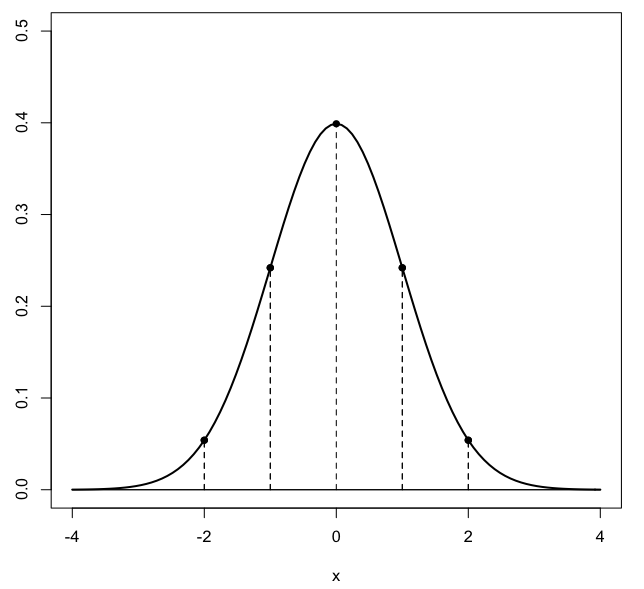
\includegraphics [scale=0.4] {gauss3.png} \end{center}
\begin{document}
\maketitle
\Large
We are interested in the value of
\[  \oint \frac{f(z)}{z - z_0} \ dz \]
in a region where there is a singularity at $z_0$ (e.g. the value of the function $\rightarrow \infty$).

Cauchy 2 says the value is the limit as $z \rightarrow z_0$, and in the previous section we showed that this simplifies the denominator to give:
\[ = i \int_0^{2\pi}  f(z) \ d \theta \]
We may choose $\rho$ as small as we like, and so we choose it very small ($\rho \rightarrow 0$) so
\[ f(z) \rightarrow f(z_0) = \text{constant} \]
and since it's constant we can bring it out of the integral!
\[  \oint \frac{f(z)}{z - z_0} \ dz = f(z_0) i \int_0^{2\pi} d \theta = 2 \pi i f(z_0) \]

\subsection*{residues}
Consider
\[ f(z) = \frac{1}{z} = \frac{z*}{zz*} = \frac{x - iy}{x^2 + y^2} \]
This function is analytic because it depends only on $z$ and not on $z*$.  If you insist, we can calculate the derivatives (note that all four derivatives have $(x^2 + y^2)^2 = d$ for the denominator).  The numerators are:
\[ u_x: \  x^2 + y^2 - 2x^2 = y^2 - x^2 \]
\[ u_y: \  -2yx \]
\[ v_x: \  -(- 2xy) = -u_y \]
\[ v_y: \  -(x^2 - y^2) = y^2 - x^2 = u_x \]

However $1/z$ "blows up" at the origin, and we say that it has a singularity or pole at the origin and the residue at the origin is equal to $1$.

The definition of the residue $R$ at $z=z_0$ where $z_0$ is a pole of $f(z)$:
\[ R(z = z_0) = \lim_{z \rightarrow z_0} \ (z - z_0) \ f(z) \]

In the case of $f(z) = 1/z$
\[  R(z = z_0) = \lim_{z \rightarrow z_0} \ \frac{z - z_0}{z} \]
\[ = \lim_{z \rightarrow 0} \ \frac{z - 0}{z}  = 1 \]

If the function were $c/z$ with $c$ a constant, then the residue would be
\[  \lim_{z \rightarrow z_0} \ (z - z_0) \  \frac{c}{z}  = c \]

As a second example, consider
\[ f(z) = \frac{1}{z + i} \cdot \frac{1}{z-i} \]
This function has poles at two points, $z = \pm i$.  As we approach $z=i$ we obtain
\[ = \frac{1}{2i} \ \frac{1}{z-i} \]
the residue at this pole is $1/2i$.

In this problem we can do:
\[ f(z) = \frac{1}{z + i} \cdot \frac{1}{z-i} =  \frac{1}{2i} \ (\frac{1}{z - i}  - \frac{1}{z+i} ) \]
To see that this is true put the fractions on the right-hand side over a common denominator:
\[ = \frac{1}{2i} \ (\frac{(z + i ) -(z-i) }{(z-i)(z+i)}) \]

so
\[ R(z = i) = \lim_{z \rightarrow i} \ (z - i) f(z) \]
\[ = \lim_{z \rightarrow i} \ (z - i) \ \frac{1}{2i} \ (\frac{1}{z - i}  - \frac{1}{z+i} ) \]
\[ = \frac{1}{2i}\  (1 - 0) = \frac{1}{2i} \]

The theory of residues is rich and (forgive me) complex, so I think I'll stop here and go study up some more.

\end{document}  
